
\documentclass{article}
\usepackage{amsmath} %Never write a paper without using amsmath for its many new commands
\usepackage{amssymb} %Some extra symbols
\usepackage{makeidx} %If you want to generate an index, automatically
\usepackage{graphicx} %If you want to include postscript graphics
%%%  \usepackage{mystyle} 
%Create your own file, mystyle.sty where you put all your own \newcommand statements
%%%
%%%
\usepackage{amscd}

\usepackage{Sweave}


%%\VignetteIndexEntry{Examples from RSEIS}

%%% \usepackage{Sweave}

\begin{document}

%%%\renewcommand\floatpagefraction{.9}
%%%\renewcommand\topfraction{.9}
%%%\renewcommand\bottomfraction{.9}
%%%\renewcommand\textfraction{.1}
%%%\setcounter{totalnumber}{50}
%%%\setcounter{topnumber}{50}
%%%\setcounter{bottomnumber}{50}

\setkeys{Gin}{width=0.9\textwidth}



\numberwithin{equation}{section}

%%%   \SweaveOpts{prefix.string=rseis}



\author{Jonathan M. Lees\\
University of North Carolina, Chapel Hill\\
Department of Geological Sciences\\
CB \#3315, Mitchell Hall\\
Chapel Hill, NC  27599-3315\\
email: jonathan.lees@unc.edu\\
ph: (919) 962-0695
}
%%  \address{University of North Carolina, Chapel Hill}
%% \contact{Jonathan M. Lees}
%% \contactaddress{Department of Geological Sciences, CB #3315, Mitchell Hall, Chapel Hill, NC  27599-3315}
%% \contactemail{jonathan.lees@unc.edu}
%% \contactphone{(919) 962-0695}
\title{RSEIS: Seismic Time Series Analysis in R}
\date{September, 2007}

\maketitle


\begin{abstract}
I present several new packages for analyzing seismic data for time
series analysis and earthquake focal mechanisms.  The packages
consists of modules that 1) read in seismic waveform data in various
common exchange formats, 2) display data as either event or continuous
recordings and 3) performs numerous standard analyses applied to
earthquake and volcano monitoring.  RSEIS is designed as a research
tool aimed at investigators who need to quickly assess large amounts
of time-series as they are related to the spatial distribution of
geologic structure and wave propagation.  In addition to time series
analysis, a spatial mapping program is included that ties waveforms
and radiation patterns to geographical data-base and mapping programs.
\end{abstract}


\section{Waveform Analysis}

The waveform module of RSEIS reads in seismic data in SEGY, SAC, AH,
UW and various ASCII formats.  The core of these modules are a set of
C programs that pass waveforms back to R and wrappers that create
lists of seismograms.  RSEIS was written primarily for use with
continuous data, so the R code is able to sort a large database
consisting of continuous data from several stations and numerous
components.  Each component of the waveform database may have a
different sample rate and may require very different handling in terms
of instrument de-convolution.  Time-windows provided by the user are
used to select off parts of the continuous data and rectify timing so
that all traces represent identical time slots.  Seismic data (binary
or ASCII format) are read into R and stored in structures that provide
a platform for object oriented manipulation of complex information
regarding earth dynamics.  In my case, I use this package to
investigate exploding volcanoes in Ecuador, Guatemala, Kamchatka and
Italy.

An initial, interactive display of the seismic records is presented to
the user and a large array of useful options are available for further
processing by buttons that surround the main display but are on the
same graphics device.  Some of the routines employed in the RSEIS
package are drawn from packages already available on the R
distribution, for example wavelet transforms - although these have
been modified to some extent to accommodate specific concerns of
seismologists. Other modules, like those dealing with focal mechanisms
and radiation patterns are original and will prove useful for
investigators searching for patterns of stress distribution in fault
regions.  


\section{Getting started}

Start by downloading packages and installing locally in the
machine being used.
The packages required by RSEIS include RPMG, and Rwave, 
and RFOC if focal mechanisms are going to be inspected.

\begin{Schunk}
\begin{Sinput}
> library(RSEIS)
> library(RPMG)
> library(Rwave)
> options(continue = " ")
\end{Sinput}
\end{Schunk}

\subsection{Example: Reventador Volcano Explosion }


There several data set that accompany RSEIS,
and these can be loaded with simple calls to data().
For example,
\begin{Schunk}
\begin{Sinput}
> data(KH)
> names(KH)
\end{Sinput}
\end{Schunk}
loads a structure that includes wave forms and other important
meta-data about the earthquake.  To see a view of this data
we call the main program and display the earthquake records as they are stored
in memory,


\begin{Schunk}
\begin{Sinput}
> STDLAB = c("DONE", "zoom in", "zoom out", "refresh", "restore", 
     "XTR", "SPEC", "SGRAM", "WLET", "FILT", "Pinfo")
> PICK.GEN(KH, SHOWONLY = FALSE, STDLAB = STDLAB)
\end{Sinput}
\end{Schunk}
\includegraphics{rseis-004}
In this example we are showing the vertical component of an explosion 
of Reventador Volcano.  The buttons at the top
are defaults chosen from a large selection of 
buttons designed to be useful for analyzing seismic data.
To zoom in on the trace, click twice on the trace with the left mouse button,
and then terminate by clicking the middle mouse.
(Clicking with the middle mouse with now left mouse clicks terminates the interactive session).
When your are finished with RSEIS windows click the ``Done'' 
button to close the window.  Avoid using the small
``x'' in the corner of the window to terminate because
R does not know you have finished yet.

You can view spectra of the signal (SPEC) , spectrograms (SGRAM) 
and wavelet transforms (WLET). To illustrate,
left click on this trace around t=1200 and t=2000, which 
windows the harmonic tremor part of this explosion.
Click middle mouse to zoom in, or
select one of the buttons at
the top to analyze the time series in the (selected) sub-window.
Choose  \emph{WLET} to show the wavelet transform of
the harmonic tremor and important time variations of the
volcano during eruption.

The PICK.GEN program is normally run in interactive mode.
In that case, once it is started R is waiting for
the user to select traces and buttons for
activating a variety of programs and analysis 
routines.
Selection of traces is accomplished by clicking on the traces,
one or more times depending 
on what is desired.
The program needs to know what to do with the 
selections once that process is over, 
usually by clicking on a button around the perimeter 
of the screen.  In the next example we will restrict the analysis
to just the vertical motion seismic data, at least for now.
If you expand the screen, you can re-arrange the buttons by
clicking on the refresh button.

PICK.GEN is a general analysis program designed for earthquake studies.
It uses the {\emph Really Poor Man's GUI} to 
navigate between seismic traces and 
various analysis procedures.
Once the program is started it waits for the user to
select on the screen a variety of operations, determined
by the user via the button selection, STDLAB.
In the main event loop, 
the user may click on the screen with the left mouse 
button to hi-light specific traces or windows in the panel.
The right mouse click terminates the clicking sequence and
a decision is made on what to do, unless a button has been clicked.
Generally, one click selects a specific trace,
two clicks specify a trace and window in that trace.
If the clicking is terminated immediately, 
before a left mouse is clicked, the program stops and returns
NULL.
If it terminates after 1 click, a refresh screen 
command is produced. If there are two or more clicks,
and no button is pressed, the last two clicks are
used to zoom in the window.

If a button is clicked, however, 
the program
uses the number of clicks to determine
which traces to process and what to do.
For example, if the ``PickWin'' button is selected,
a new PICK.GEN is spawned where the program 
gathers all the components for that station, Usually Vertical, North and East,
although in the presence of acoustic channels they will also be displayed.
The new window is called with a new set of Buttons
set up specifically for picking the P, S and Acoustic arrivals.
Once that window is finished, focus reverts to the main 
window and the new picks are registered.
Selecting the ``SavePF'' button will save the
new picks to a file for later use.

As another example, if the user clicks twice in a trace panel,
and then selects the WLet Button, a wavelet transform
of the selected time window is calculated and 
a special new screen is exposed where the 
user is now focused until that session is finished by
clicking ``Done''.

Each Button has different properties based on the 
requirements for that process.  Some buttons 
expect more than one click to operate properly, others 
are simple buttons that control the look and feel of the 
panel. For example, the ``restore'' button
reverts the panel to its original time window.
It can be pressed any time and the 
window will redraw and resize.
Each button includes a small set of instructions
designed to accomplish a specific task.
There are many buttons currently defined, some described below, and 
there is mechanism for users to  make their own
on the fly.


\subsection{Example: Coso Geothermal Event }

\begin{Schunk}
\begin{Sinput}
> data(GH)
> numstas = length(GH$STNS)
\end{Sinput}
\end{Schunk}

In this example, taken from the geothermal field 
at Coso, California, there are 49 stations,
most of which have three components (Vertical, North and East),
although there are a couple of stations that are missing
some of the components.  This situation is not 
atypical of earthquake seismic data recorded in the field.
If we show only the vertical component traces,
The plot is more manageable and easier to view:
\begin{Schunk}
\begin{Sinput}
> verts = which(GH$COMPS == "V")
> STDLAB = c("DONE", "QUIT", "NEXT", "PREV", "zoom in", "zoom out", 
     "refresh", "restore", "SavePF", "PickWin", "XTR", "SPEC", 
     "SGRAM", "WLET", "FILT", "Pinfo", "WINFO", "PTS", "YPIX", 
     "WPIX")
> PICK.GEN(GH, sel = verts, STDLAB = STDLAB, SHOWONLY = TRUE)
\end{Sinput}
\end{Schunk}
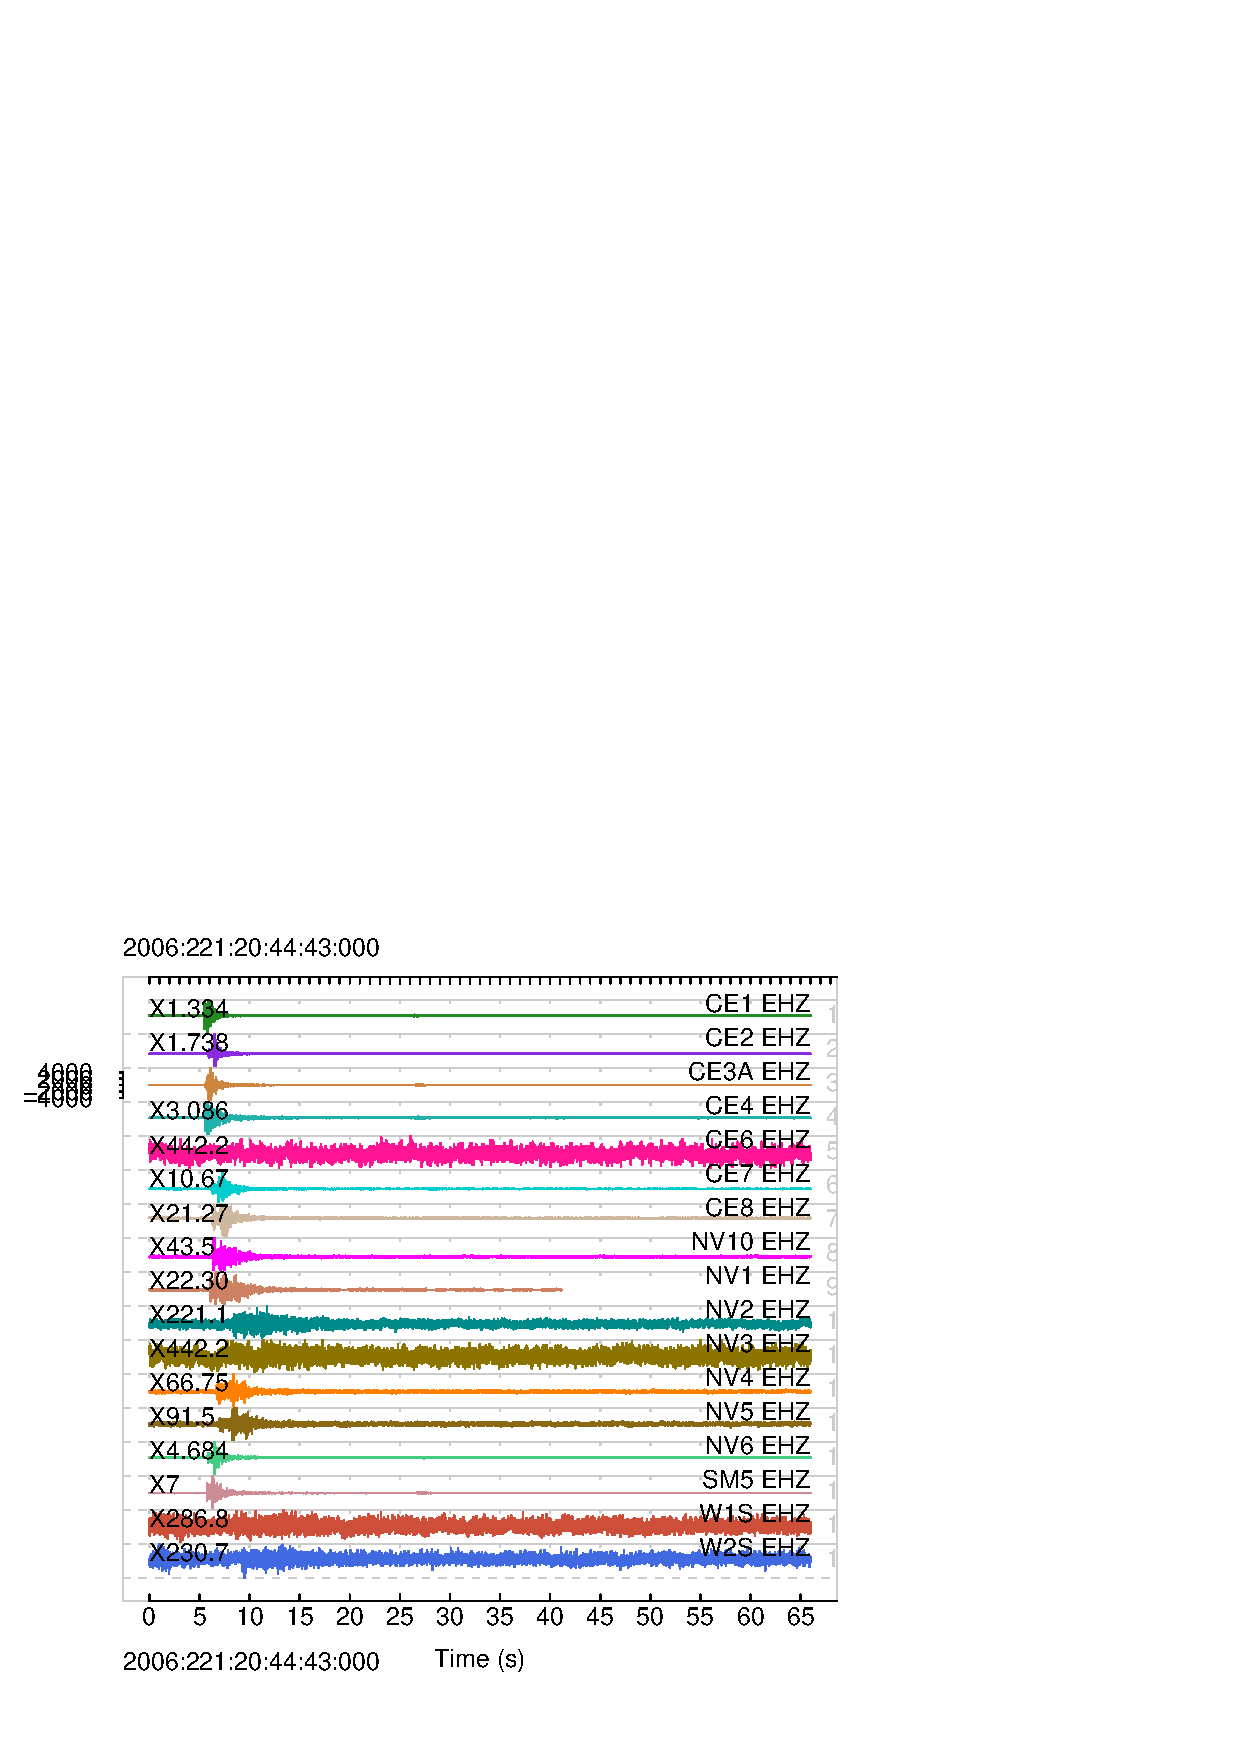
\includegraphics{rseis-006}




We see that the stations here are 'mixed up', i.e. arriving at different times.
\begin{Schunk}
\begin{Sinput}
> vertord = getvertsorder(GH$pickfile, GH)
> PICK.GEN(GH, sel = vertord$sel, STDLAB = STDLAB, SHOWONLY = FALSE)
\end{Sinput}
\end{Schunk}
\includegraphics{rseis-007}

A seismic event is usually stored as a combination
of waveform information and meta-date associated with
the phase arrivals.  Phase arrivals are
commonly called ``picks'' since and analyst 
had to pick the arrival times from a representation
of the seismic signals, either on a computer or on a paper
record.
The picks are stored in RSEIS 
in a list structure called pickfile
which is an optional  component of the name waveform structure.
The pickfile structure is a list comprising several
sub-lists with important information associated with
stations and the event (earthquake) source.
\begin{Schunk}
\begin{Sinput}
> names(GH$pickfile)
\end{Sinput}
\begin{Soutput}
 [1] "PF"       "AC"       "LOC"      "MC"       "STAS"     "LIP"     
 [7] "E"        "F"        "filename" "UWFILEID" "comments" "OSTAS"   
[13] "H"        "N"       
\end{Soutput}
\end{Schunk}
For now we consider the most relevant 
meta-data, 
\begin{Schunk}
\begin{Sinput}
> names(GH$pickfile$STAS)
\end{Sinput}
\begin{Soutput}
 [1] "tag"   "name"  "comp"  "c3"    "phase" "sec"   "err"   "pol"   "flg"  
[10] "res"   "lat"   "lon"   "z"    
\end{Soutput}
\end{Schunk}
which is a list of vectors, 
one for each meta-datum and one element
each for each station that has meta-data.
We see in this example there are a couple of picks per station,
some picks are on the vertical components and some
are on the North component or East, there
are P and S-wave phase picks.
\begin{Schunk}
\begin{Sinput}
> data.frame(cbind(name = GH$pickfile$STAS$name, comp = GH$pickfile$STAS$comp, 
     phase = GH$pickfile$STAS$phase, time = GH$pickfile$STAS$sec, 
     lat = GH$pickfile$STAS$lat, lon = GH$pickfile$STAS$lon))
\end{Sinput}
\begin{Soutput}
   name comp phase   time       lat         lon
1   CE1    V     P 48.476   36.0131   -117.8025
2   CE4    V     P 48.532   35.9998   -117.8023
3  CE3A    V     P   48.6   36.0145   -117.8198
4   SM5    V     P  48.74  35.99965 -117.830261
5   NV6    V     P 48.812   35.9823   -117.8076
6   CE2    V     P 48.876   36.0337   -117.7883
7   NV1    V     P 49.072   35.9827   -117.7649
8   CE7    V     P 49.176    36.053   -117.8046
9  NV10    V     P 49.312 35.999056 -117.745194
10  CE8    V     P 49.292   36.0512   -117.8387
11  NV4    V     P 49.688   36.0477   -117.7403
12  NV5    V     P 49.996   36.0839   -117.7536
13  NV2    V     P 51.292   36.0255   -117.6213
14  CE1    N     S 48.752   36.0131   -117.8025
15  CE4    N     S 48.872   35.9998   -117.8023
16 CE3A    N     S 48.908   36.0145   -117.8198
17  SM5    N     S 49.216  35.99965 -117.830261
18  NV6    N     S 49.372   35.9823   -117.8076
19  CE2    N     S 49.444   36.0337   -117.7883
20  CE6    N     S 49.704 36.033665 -117.772726
21  CE7    N     S 49.876    36.053   -117.8046
22  CE8    E     S 50.316   36.0512   -117.8387
23  NV4    N     S 50.984   36.0477   -117.7403
24  NV5    N     S  51.28   36.0839   -117.7536
\end{Soutput}
\end{Schunk}
We also store event information:
\begin{Schunk}
\begin{Sinput}
> names(GH$pickfile$LOC)
\end{Sinput}
\begin{Soutput}
 [1] "yr"     "mo"     "dom"    "hr"     "mi"     "sec"    "jd"     "lat"   
 [9] "lon"    "z"      "mag"    "gap"    "delta"  "rms"    "hozerr"
\end{Soutput}
\end{Schunk}

Using this information we can associate the 
p-pick with the waveforms, match the timing information
and plot together.
finally we add the picks to the section:
\begin{Schunk}
\begin{Sinput}
> apx = uwpfile2ypx(GH$pickfile)
> PICK.GEN(GH, sel = vertord$sel, APIX = apx, STDLAB = STDLAB, 
     SHOWONLY = FALSE, velfile = VELMOD1D, )
\end{Sinput}
\end{Schunk}
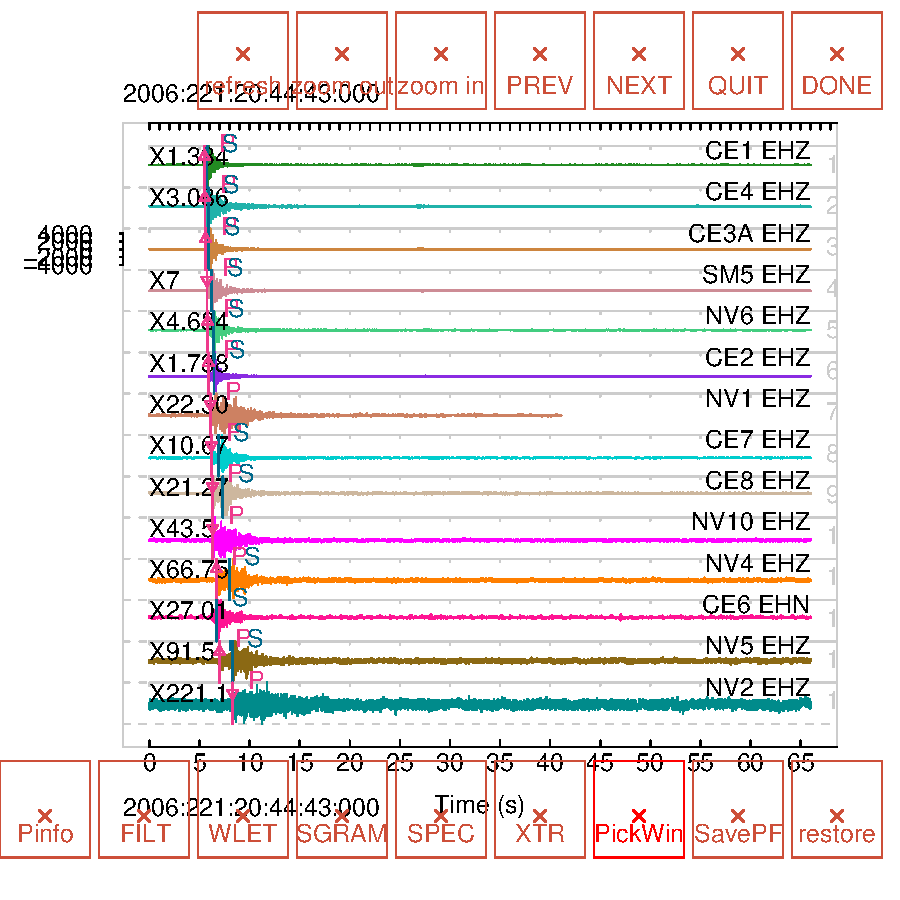
\includegraphics{rseis-012}

Brief documentation for buttons in the PICK.GEN
program can be seen by calling the documentation function,
either for a specific button 

\begin{Schunk}
\begin{Sinput}
> PICK.DOC("WLET")
\end{Sinput}
\begin{Soutput}
[1] "WLET: wavelet analysis"
\end{Soutput}
\end{Schunk}
or for 
all possible buttons.
\begin{Schunk}
\begin{Sinput}
> PICK.DOC()
\end{Sinput}
\begin{Soutput}
$DONE
[1] "DONE: Close Window and Finish"

$MARK
[1] "MARK Mark a Specific Trace"

$restore
[1] "restore: restore the window traces to full screen"

$`zoom out`
[1] "zoom out: Zoom out by a percent"

$`zoom in`
[1] "zoom in: Zoom in  by a percent"

$Left
[1] "Left: Shift Left by a percent"

$Right
[1] "Right: Shift Right by a percent"

$SCALE
[1] "SCALE: Toggle: SCALE by trace or scale by Window"

$Postscript
[1] "Postscript: create a Postscript file"

$AUTOP
[1] "AUTOP: Automatic picking on one trace"

$AUTOPALL
[1] "AUTOPALL: Automatic picking on all traces in window"

$DETECT
[1] "DETECT: signal detection using automated picking"

$XTR
[1] "XTR: extract a single trace and return at end of session"

$SIG
[1] "SIG: pulse analysis (chugging)"

$SPEC.old
[1] "SPEC.old: "

$SPEC
[1] "SPEC: MTM spectrum in separate window with options"

$SGRAM
[1] "SGRAM: spectrogram window"

$WLET
[1] "WLET: wavelet analysis"

$FILT
[1] "FILT: filter a trace with a set of choices"

$BRUNE
[1] "BRUNE: do brune model analysis for short period data, save meta-data"

$DETAIL
[1] "DETAIL: pick details of first arrivals and save meta data"

$PTS
[1] "PTS: toggle points option, plot each point in time series"

$MMARKS
[1] "MMARKS: Unused"

$PMOT
[1] "PMOT: particle motion hodogram, must have three components in the window"

$STERNET
[1] "STERNET: plot an equal area steronet with the points of the 3-comp seismogram"

$GTAZI
[1] "GTAZI: SVD particle motion in windows (needs 3Comp seis)"

$ENVLP
[1] "ENVLP: get envelope of a windowed time series"

$Pinfo
[1] "Pinfo: pick information"

$XCOR
[1] "XCOR: cross correlation of traces"

$PHLAG
[1] "PHLAG: calculate the phase lag between traces based on cross spectrum"

$YPIX
[1] "YPIX: Y picking"

$WPIX
[1] "WPIX: Window picks"

$EDIX
[1] "EDIX: edit window picks"

$NOPIX
[1] "NOPIX: erase all previous picks"

$REPIX
[1] "REPIX: restore previously erased picks"

$FLIP
[1] "FLIP: Flip polarity of traces"

$`3COMP`
[1] "3COMP: find all componenets of this station and plot in separate window"

$DOC
[1] "DOC: print Documentation"
\end{Soutput}
\end{Schunk}


\subsection{Example: SunSpots}

One standard data set included in the R
Distribution is the 
sunspot data.  As an example of RSEIS we can read this time series in and plot it using the
same code introduced above.
\begin{Schunk}
\begin{Sinput}
> data(sunspots)
> ES = prep1wig(wig = sunspots, dt = 1/12, sta = "STA", comp = "CMP", 
     units = "UNITS")
> EH = prepSEIS(ES)
> STDLAB = c("DONE", "zoom in", "zoom out", "refresh", "restore", 
     "XTR", "SPEC", "SGRAM", "WLET", "FILT", "Pinfo")
> xx = PICK.GEN(EH, STDLAB = STDLAB, SHOWONLY = TRUE)
\end{Sinput}
\end{Schunk}
\includegraphics{rseis-015}


\begin{Schunk}
\begin{Sinput}
> a = list(y = EH$JSTR[[1]], dt = EH$dt[1])
> Mspec = mtapspec(a$y, a$dt, klen = 1024, MTP = list(kind = 1, 
     nwin = 5, npi = 3, inorm = 0))
> f = Mspec$freq
> amp = Mspec$spec[1:length(f)]
> ma = amp
> displ = ma
> f1 = 0.01
> f2 = 1/(2 * EH$dt[1])
> flag = f >= f1 & f <= f2
> plxy = "xy"
> plot(range(f[flag]), range(displ[flag]), type = "n", log = plxy, 
     axes = FALSE, xlab = "Hz", ylab = "Spec")
> lines(f[flag], displ[flag], col = 1, lty = 1)
> axis(2, las = 2)
> axis(1)
> box()
> L = list()
> L$x = c(0.0939105803154482, 0.183351679178275, 0.350333785192083)
> L$y = c(31166.8951116052, 7536.36156151748, 2370.29538151056)
> abline(v = L$x, lty = 2, col = grey(0.8))
> text(L$x, rep(max(range(displ[flag])), length(L$x)), labels = round((1/L$x)), 
     xpd = TRUE, srt = 45, adj = c(0, 0))
\end{Sinput}
\end{Schunk}


\subsection{Example: Climate Change}

As a final example showing how RSEIS might be used for 
arbitrary time series, unrelated to 
seismic data, consider the famous 
Delta-O18 time series.  By windowing the 
time sereis and looking at the 
spectrum one can immediately see the 
Milankovitch cycles at (approximately) 100K, 41K and 20K periods.

\begin{Schunk}
\begin{Sinput}
> data(OH)
> xx = PICK.GEN(OH, sel = which(OH$COMPS == "V"), STDLAB = STDLAB, 
     SHOWONLY = TRUE)
\end{Sinput}
\end{Schunk}
\includegraphics{rseis-017}

\begin{Schunk}
\begin{Sinput}
> a = list(y = OH$JSTR[[1]], dt = OH$dt[1])
> Mspec = mtapspec(a$y, a$dt, klen = 1024, MTP = list(kind = 1, 
     nwin = 5, npi = 3, inorm = 0))
> f = Mspec$freq
> amp = Mspec$spec[1:length(f)]
> ma = amp
> displ = ma
> f1 = 0.01
> f2 = 1/(2 * EH$dt[1])
> flag = f >= f1 & f <= f2
> plxy = "xy"
> plot(range(f[flag]), range(displ[flag]), type = "n", log = plxy, 
     axes = FALSE, xlab = "Hz", ylab = "Spec")
> lines(f[flag], displ[flag], col = 1, lty = 1)
> axis(2, las = 2)
> axis(1)
> box()
> u = par("usr")
> L = list()
> L$x = c(0.242745864538716, 0.423063797271721, 0.447439169221329, 
     0.529320129815409, 0.100457805181183)
> L$y = c(37.4392793655756, 19.0231348719557, 15.6564640841027, 
     15.0862607475168, 40.6986171075992)
> abline(v = L$x, lty = 2, col = grey(0.8))
> text(L$x, rep(max(range(displ[flag])), length(L$x)), labels = round(10000 * 
     (1/L$x)), xpd = TRUE, srt = 45, adj = c(0, 0))
\end{Sinput}
\end{Schunk}
\includegraphics{rseis-018}



To illustrate the effects of comparing numerous filters to 
a specific volcanic explosions event,


\begin{Schunk}
\begin{Sinput}
> data(KH)
> dt = KH$dt[1]
> y = KH$JSTR[[1]]
> y = y[1:50000]
> y = y - mean(y)
> x = seq(from = 0, by = dt, length = length(y))
> fl = rep(1/100, 5)
> fh = 1/c(4, 3, 2, 1, 0.5)
> FILT.spread(x, y, dt, fl = fl, fh = fh, sfact = 1, WIN = NULL, 
     PLOT = TRUE, TIT = NULL, TAPER = 0.05, POSTTAPER = 0.1)
\end{Sinput}
\end{Schunk}
\includegraphics{rseis-019}




\end{document}



